\Exercise[number={4}]
Consider the following HMM:
\begin{figure}[H]
    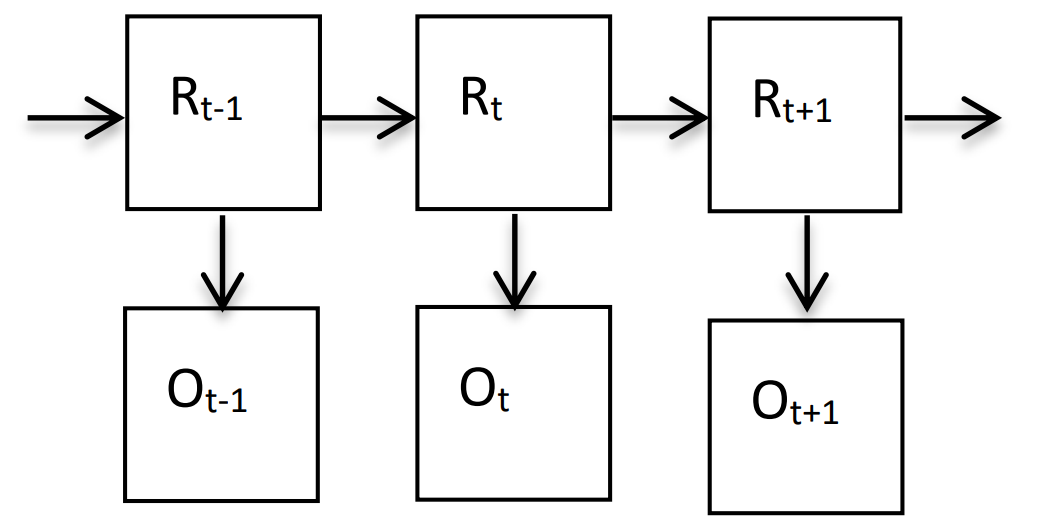
\includegraphics[scale=0.45]{E_3}
    \centering
\end{figure}
Which relates the observation that it rains on day (\(R_t=yes\))
with the observation that it has been raining the day before and that people
carry an umbrella, \(O_t = yes\).\\
You know that \(Pr(R_t=yes|R_{t-1}=yes)=0.8\) and that
\(Pr(R_t=yes|R_{t-1}=no)=0.1\). You also know that
\(Pr(O_t=yes|R_t=yes)=0.9\), \(Pr(O_t=yes|R_t=no)=0.3\) and
\(Pr(R_1=yes)=0.5\).\\
Calculate the probability to have rain on day 3 after having observed
people carrying umbrella (\(O_t=yes\)) for three consecutive days.

\Answer[number={4}]
First of all, let's compute explicitly all the necessary probabilities:
\begin{align*}
    \begin{matrix}
        Pr(R_1=yes)=0.5 && \Rightarrow && Pr(R_1=no)=1-0.5=0.5\\
        Pr(R_{t}=yes|R_{t-1}=yes)=0.8 && \Rightarrow && Pr(R_{t}=no|R_{t-1}=yes)=1-0.8=0.2\\
        Pr(R_{t}=yes|R_{t-1}=no)=0.1 && \Rightarrow && Pr(R_{t}=no|R_{t-1}=no)=1-0.1=0.9\\
        Pr(O_{t}=yes|R_{t}=yes)=0.9 && \Rightarrow && Pr(O_{t}=no|R_{t}=yes)=1-0.9=0.1\\
        Pr(O_{t}=yes|R_{t}=no)=0.3 && \Rightarrow && Pr(O_{t}=no|R_{t}=no)=1-0.3=0.7
    \end{matrix}
\end{align*}
The probability to have rain on day 3 after having observed
people carrying umbrella for three consecutive days can be summarized as:
\begin{align*}
    Pr(R_3=yes|O_{1:3}=yes)
    =Pr(R_3=yes|O_1=yes,O_2=yes,O_3=yes)
\end{align*}
In order to proceed, this conditional probability requires to be transformed
into a joint probability:
\begin{align*}
    Pr(R_3=yes|O_1=yes,O_2=yes,O_3=yes)
    =\frac{Pr(R_3=yes,O_1=yes,O_2=yes,O_3=yes)}{Pr(O_1=yes,O_2=yes,O_3=yes)}
\end{align*}
Now let's compute numerator (\(\mathcal{N}\)) and denominator (\(\mathcal{D}\)) values
separatelely. Let's start from the numerator:
\begin{align*}
    \mathcal{N}
    &=Pr(R_3=yes,O_1=yes,O_2=yes,O_3=yes)\\
    &=Pr(R_1,R_2,R_3=yes,O_1=yes,O_2=yes,O_3=yes)\\
    &=\sum_{R_1}\sum_{R_2}Pr(R_1)Pr(O_1=yes|R_1)Pr(R_2|R_1)Pr(O_2=yes|R_2)Pr(R_3=yes|R_2)Pr(O_3=yes|R_3=yes)
\end{align*}
\(R_1\) and \(R_2\) can assume two values each, meaning that there are
\(2^2=4\) possible combinations. Let's compute the respective probabilities:
\begin{align*}
    &1)R_1=yes, R_2=yes
    &\Rightarrow
    0.5\cdot0.9\cdot0.8\cdot0.9\cdot0.8\cdot0.9=0.23328\\
    &2)R_1=yes, R_2=no
    &\Rightarrow
    0.5\cdot0.9\cdot0.2\cdot0.3\cdot0.1\cdot0.9=0.00243\\
    &3)R_1=no, R_2=yes
    &\Rightarrow
    0.5\cdot0.3\cdot0.1\cdot0.9\cdot0.8\cdot0.9=0.00972\\
    &4)R_1=no, R_2=no
    &\Rightarrow
    0.5\cdot0.3\cdot0.9\cdot0.3\cdot0.1\cdot0.9=0.00365
\end{align*}
Therefore, \(\mathcal{N}=0.23328+0.00243+0.00972+0.00365\simeq0.2491\).\\
The denominator can be calculated by exploiting the same approach, however
\(R_3\) cannot be assumed always positive (as done in the numerator case),
in fact:
\begin{align*}
    \mathcal{D}
    &=Pr(O_1=yes,O_2=yes,O_3=yes)\\
    &=Pr(R_1,R_2,R_3,O_1=yes,O_2=yes,O_3=yes)\\
    &=Pr(R_1,R_2,R_3=yes,O_1=yes,O_2=yes,O_3=yes)+\\
    &\quad +Pr(R_1,R_2,R_3=no,O_1=yes,O_2=yes,O_3=yes)\\
    &=\mathcal{N}+Pr(R_1,R_2,R_3=no,O_1=yes,O_2=yes,O_3=yes)\\
    &=\mathcal{N}+\mathcal{D}'
\end{align*}
Let's now compute the part of the denominator accounting for \(R_3=no\):
\begin{align*}
    \mathcal{D}'
    &=Pr(R_1,R_2,R_3=no,O_1=yes,O_2=yes,O_3=yes)\\
    &=\sum_{R_1}\sum_{R_2}Pr(R_1)Pr(O_1=yes|R_1)Pr(R_2|R_1)Pr(O_2=yes|R_2)Pr(R_3=no|R_2)Pr(O_3=yes|R_3=no)
\end{align*}
Notice that if \(R_3\) is not known there are \(2^3=8\) possible cases, four
of them with \(R_3=yes\) (the ones computed in the numerator case) and four
with \(R_3=no\), which are to be computed below:
\begin{align*}
    &1)R_1=yes, R_2=yes
    &\Rightarrow
    0.5\cdot0.9\cdot0.8\cdot0.9\cdot0.2\cdot0.3=0.01944\\
    &2)R_1=yes, R_2=no
    &\Rightarrow
    0.5\cdot0.9\cdot0.2\cdot0.3\cdot0.9\cdot0.3=0.00729\\
    &3)R_1=no, R_2=yes
    &\Rightarrow
    0.5\cdot0.3\cdot0.1\cdot0.9\cdot0.2\cdot0.3=0.00081\\
    &4)R_1=no, R_2=no
    &\Rightarrow
    0.5\cdot0.3\cdot0.9\cdot0.3\cdot0.9\cdot0.3=0.01094
\end{align*}
Therefore, \(\mathcal{D}=\mathcal{N}+0.01944+0.00729+0.00081+0.01094=0.28758\).\\
Finally, \(Pr(R_3=yes|O_{1:3}=yes)=\frac{\mathcal{N}}{\mathcal{D}}=\frac{0.2491}{0.28758}=0.8662\simeq86.6\%\), a reasonable value.